\begin{homework}
  %--------------------------------------------------------------------
  \question How many independent quantities are necessary to fully describe a state of matter?
  %--------------------------------------------------------------------
  \question Define the following: phase, state, property, process
  %--------------------------------------------------------------------
  \question Two kilograms of water at 25°C are placed in a piston cylinder device under 3.2 MPa pressure. Heat is added to the water at constant pressure until the temperature of the fluid reaches 350°C (State (2)). Determine the final volume of the fluid at state (2). $\answer{[0.08508\ {\rm m^3}/{\rm kg}]}$
   %--------------------------------------------------------------------
  \question A piston-cylinder device contains a saturated mixture of steam and water having a total mass of 0.5 kg at a pressure of 160 kPa and an initial volume of 100 liters. Heat is then added and the fluid expands at constant pressure until it reaches a saturated vapor state.
\begin{questionparts}
\item Draw a diagram representing the process showing the initial and final states of the system.

\item Sketch this process on a P-v diagram with respect to the saturation lines, critical point, and relevant constant temperature lines, clearly indicating the initial and final states.

\item Determine the initial quality and temperature of the fluid mixture prior to heating. {\color{red} [$x_1$ = 0.182, $T_1$ = 113.3°C]}

\item Determine the final volume of the steam after heating. {\color{red} [0.546 $\rm m^3$ (546 liters)]}
\end{questionparts}
%--------------------------------------------------------------------
\question A pressure cooker allows much faster (and more tender) cooking by maintaining a higher boiling temperature of the water inside. It is well sealed, and steam can only escape through an opening on the lid, on which sits a metal petcock. When the pressure overcomes the weight of the petcock, the steam escapes, maintaining a constant high pressure while the water boils.

\begin{center}
  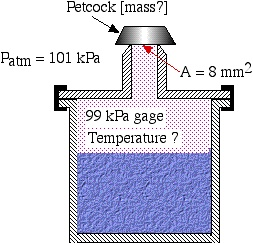
\includegraphics[width=0.4\textwidth]{press_cooker}
\end{center}
  
Assuming that the opening under the petcock has an area of 8 $\rm mm^2$, determine:

\begin{questionparts}
\item the mass of the petcock required in order to maintain an operating pressure of 99 kPa gauge. {\color{red}[80.7 g]}

\item the corresponding temperature of the boiling water. {\color{red}[120.2°C]}
\end{questionparts}
Note: Assume that the atmospheric pressure is 101 kPa. Draw a free body diagram of the petcock.

%--------------------------------------------------------------------
\question Consider a rigid container having a volume of 100 liters, filled with steam at an initial state of 400 kPa and 300°C. The steam is then cooled until it reaches a temperature of 90°C.

\begin{questionparts}
\item Draw a diagram representing the process showing the initial and final states of the system.

\item Using steam tables determine the mass of steam in the container. {\color{red} [0.153 kg]}

\item Using the ideal gas equation of state determine the mass of steam in the container. {\color{red} [0.151 kg]}
Determine the percentage error of using this method compared to that of using the steam tables. {\color{red}[1\%]}

\item Sketch this process on a $T$-$v$ (temperature-specific volume) diagram with respect to the saturation lines, critical point, and relevant constant pressure lines, clearly indicating the initial and final states.

\item Using steam tables determine the final pressure and quality of the fluid mixture after cooling. {\color{red}[70.2 kPa, $x$ = 0.277]}
\end{questionparts}
Note: The critical point data and ideal gas constant for steam can be found on the first page of the steam tables.

%--------------------------------------------------------------------

\question An automobile tire with a volume of 100 liters is inflated to a gauge pressure of 210 kPa. Determine:
\begin{questionparts}
\item the mass of air in the tire if the temperature is 20°C {\color{red} [$m$ = 0.369 kg]}
\item the increase in gauge pressure if the temperature in the tire reaches 50°C \\{\color{red} [$p_{2,gage}=$242 kPa]}
\end{questionparts}
Assume that atmospheric pressure is 100 kPa.

%--------------------------------------------------------------------

\question Compressed air is commonly used to power a large variety of power tools.  Lowe's sells an air compressor that can fill an 8-gallon tank to 160 psi. At a temperature of 70°F, determine the mass of the air inside a full 8-gallon tank.  Let $p_{atm} = 14.7$ psi.
\begin{questionparts}

\item Use the ideal gas law (you will need to do a lot of unit conversions for this). \\{\color{red} [0.429 kg]}

\item Find the compressibility factor.  How far off is your analysis above? {\color{red} [0.99]}

\end{questionparts}
\end{homework}
